% Source: physical PDF p. 139 (printed p. 116). Coverage: Figure 18.1 and complete caption. Uncertainty: none; vector geometry reconstructed from the rendered scan.
\begin{figure}[htbp]
 \centering
 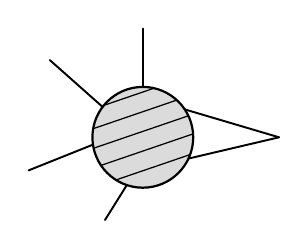
\begin{tikzpicture}[x=1cm,y=1cm,line cap=round,line join=round]
  \draw[line width=0.7pt] (0,1.38) -- (0,0.62);
  \draw[line width=0.7pt] (-1.18,0.98) -- (-0.47,0.35);
  \draw[line width=0.7pt] (-1.45,-0.42) -- (-0.60,-0.08);
  \draw[line width=0.7pt] (-0.48,-1.05) -- (-0.18,-0.57);
  \draw[line width=0.7pt] (0.48,0.37) -- (1.73,0);
  \draw[line width=0.7pt] (0.58,-0.27) -- (1.73,0);
  \fill[gray!28] (0,0) circle[radius=0.64];
  \begin{scope}
   \clip (0,0) circle[radius=0.64];
   \foreach \a in {-1.25,-1.00,...,1.25}
    \draw[line width=0.45pt] (-0.95,\a) -- (0.95,{\a+0.65});
  \end{scope}
  \draw[line width=0.8pt] (0,0) circle[radius=0.64];
 \end{tikzpicture}
 \renewcommand{\thefigure}{18.1}
 \caption{Momentum-space Feynman diagrams for the matrix element of the operator $\int \dd^4x\,\exp(-\ii p\cdot x)\,\phi^2(x)$ in the theory of an elementary scalar field $\phi(x)$. The cross-hatched disk represents the sum of diagrams with the indicated external lines. Apart from the pair of external lines that meet in a $\phi^2$ vertex, the other external lines attached to the disk represent the particles in the initial and final states between which the matrix element is evaluated.}
 \label{fig:18.1}
\end{figure}
